\documentclass[11pt]{article}
\usepackage[margin=0.7in]{geometry}
\usepackage{tikz,longtable,hyperref}
\setlength{\parindent}{0pt}\setlength{\parskip}{7pt}
\begin{document}
\raggedright\sloppy
{\LARGE Mathematical experiment preparation: gate software and published runtime}\\[5pt]
2026-10-29T23:58:29Z\\
Public synthetic known-answer mathematical research. Evidence observations only; no judgments, new cohort executions or qualification.

Zero executions refers to this named plan-only input, not historical experiments. Per-source software scopes are distinct and counts are never pooled.
\section*{Plan-only observations}
\begin{center}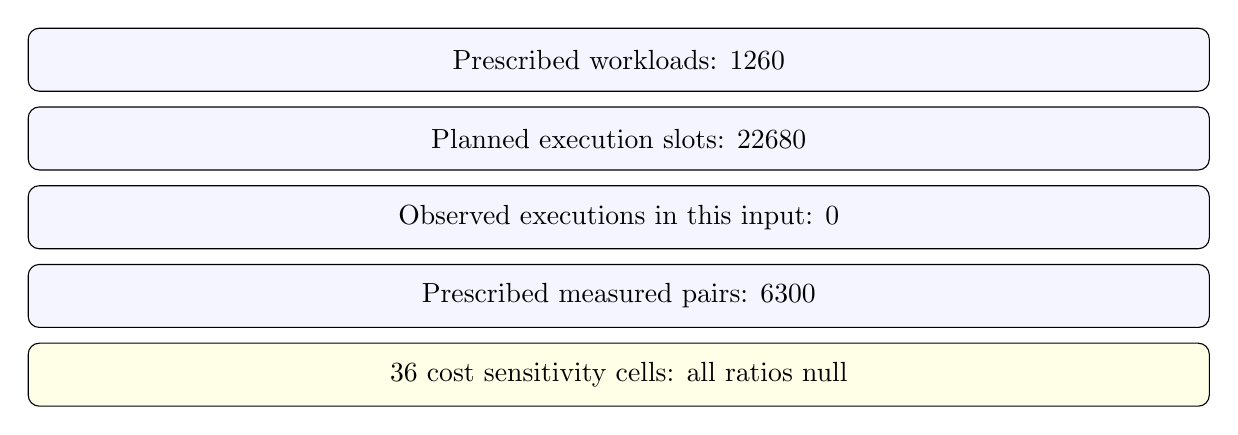
\begin{tikzpicture}
\node[draw,rounded corners,fill=blue!4,minimum width=15cm,minimum height=0.8cm] at (0,-0) {Prescribed workloads: 1260};
\node[draw,rounded corners,fill=blue!4,minimum width=15cm,minimum height=0.8cm] at (0,-1) {Planned execution slots: 22680};
\node[draw,rounded corners,fill=blue!4,minimum width=15cm,minimum height=0.8cm] at (0,-2) {Observed executions in this input: 0};
\node[draw,rounded corners,fill=blue!4,minimum width=15cm,minimum height=0.8cm] at (0,-3) {Prescribed measured pairs: 6300};
\node[draw,rounded corners,fill=yellow!10,minimum width=15cm,minimum height=0.8cm] at (0,-4) {36 cost sensitivity cells: all ratios null};
\end{tikzpicture}\end{center}
Diagram rather than a performance graph: this input contains no observed empirical ratios. Counts are read from source [plan]; no rates or uncertainty estimates are inferred.
Warmup execution slots prescribed: 3780. No empirical cost ratio is available in this snapshot. Software validation and prepared inputs do not constitute independent protocol, binary, resource or launch admission.
\section*{Scoped source observations}
\textbf{[gate-software]} Software validation only. The full 1260 design remains intact; the exact p739 gate has 60 planned targets. Counts refer to software tests, not empirical targets.\\
export\_private\_units: 37\\
export\_production\_scope\_tests: 2\\
native\_cli\_tests: 1\\
native\_unit\_tests: 29\\
planned\_gate\_pairs: 300\\
planned\_gate\_slots: 1080\\
planned\_gate\_targets: 60\\
qualified\_ratios: null\\
solver\_executions: 0\\
\textbf{[gate-review]} Independent read-only software scope review. No mathematical workload, timing observation or cost ratio was replayed; source-commit binding is a separate record.\\
findings: []\\
review\_result: "no\_concrete\_gate\_logic\_defect\_found"\\
solver\_executions: 0\\
source\_commit: "99b10d5c6f3f5f3fcdea8fb5a9484ac3a9ec6ff0"\\
\textbf{[controller-publication]} Retained CodeBuild source-update receipt. The CloudFormation change set was not executed. Its source parameters remain old, so later stack changes require reconciliation.\\
change\_set\_executed: false\\
experiment\_launched\_at\_receipt: false\\
inline\_policy\_unchanged: true\\
other\_project\_properties\_unchanged: true\\
source\_update\_completed: true\\
\textbf{[image-publication]} Approved FROM/COPY image publication and stopped-container extraction. Elapsed time is infrastructure publication/verification, not mathematical performance. No workload was started.\\
historical\_qualification\_transferred: false\\
image\_digest\_pull\_verified: true\\
publication\_seconds: 122\\
runtime\_bytes\_equal: true\\
solver\_executions: 0\\
stopped\_extraction\_verified: true\\
\textbf{[bytebinding-audit]} Separate check of retained archive and image bytes plus API receipts. This auditor also published the image; it is not an independent-personnel audit or live cluster check.\\
archive\_readback\_matches: true\\
cloud\_mutations\_in\_audit: 0\\
empirical\_ratios: null\\
image\_runtime\_bytes\_equal: true\\
inline\_policy\_bytes\_equal: true\\
source\_only\_project\_match: true\\
\section*{Evidence and limits}
No software test count is an empirical target count. Missing costs stay null. Resource authorization is limited to its explicit source scope; no budget, deadline, infrastructure approval or independent review is inferred. The prior 19:06 report and its Python generator remain historical artifacts; new reports use this native renderer.
\small
\textbf{[plan]} named plan-only input; not historical experiments\\
\texttt{/\allowbreak{}home/\allowbreak{}ec2-user/\allowbreak{}crypto-pencil-signed-graph-20261029/\allowbreak{}research/\allowbreak{}pencil\_large\_prime\_20261029/\allowbreak{}validation/\allowbreak{}accounting/\allowbreak{}aggregate/\allowbreak{}actual-plan-only-summary-final.json}\\
SHA256: \texttt{9c0d055e2af7f6f79ce201b9b0c2a22691da0af55e8f6f127acec7070bb7e665}\\
\textbf{[gate-software]} Software validation only. The full 1260 design remains intact; the exact p739 gate has 60 planned targets. Counts refer to software tests, not empirical targets.\\
\texttt{/\allowbreak{}home/\allowbreak{}ec2-user/\allowbreak{}crypto-pencil-signed-graph-20261029/\allowbreak{}research/\allowbreak{}pencil\_large\_prime\_20261029/\allowbreak{}validation/\allowbreak{}gate60\_analysis\_20261029/\allowbreak{}receipt.json}\\
SHA256: \texttt{14a482e87682761cbe6a29b777714fb5dc7c700cb5152745a7aa3a859e232d8e}\\
\textbf{[gate-review]} Independent read-only software scope review. No mathematical workload, timing observation or cost ratio was replayed; source-commit binding is a separate record.\\
\texttt{/\allowbreak{}home/\allowbreak{}ec2-user/\allowbreak{}crypto-pencil-signed-graph-20261029/\allowbreak{}research/\allowbreak{}pencil\_large\_prime\_20261029/\allowbreak{}validation/\allowbreak{}publication\_binding\_audit\_20261029T2358Z/\allowbreak{}gate-independent-review.json}\\
SHA256: \texttt{8d53fd6fde1a9b2f30608620aa64b1e72901b4ce84a187d42755e8cca0f33140}\\
\textbf{[controller-publication]} Retained CodeBuild source-update receipt. The CloudFormation change set was not executed. Its source parameters remain old, so later stack changes require reconciliation.\\
\texttt{/\allowbreak{}home/\allowbreak{}ec2-user/\allowbreak{}crypto-pencil-signed-graph-20261029/\allowbreak{}research/\allowbreak{}pencil\_large\_prime\_20261029/\allowbreak{}validation/\allowbreak{}controller\_publication\_20261029/\allowbreak{}receipt.json}\\
SHA256: \texttt{ef0fc0a6f3665173a769187c7a130561cc727051f539ae3862c2c9367ab13980}\\
\textbf{[image-publication]} Approved FROM/COPY image publication and stopped-container extraction. Elapsed time is infrastructure publication/verification, not mathematical performance. No workload was started.\\
\texttt{/\allowbreak{}home/\allowbreak{}ec2-user/\allowbreak{}crypto-pencil-signed-graph-20261029/\allowbreak{}research/\allowbreak{}pencil\_large\_prime\_20261029/\allowbreak{}validation/\allowbreak{}controller\_publication\_20261029/\allowbreak{}image-publication-receipt.json}\\
SHA256: \texttt{f5fa87421c688ac0fda54105306c5442cae8229287d583469a6da347c09b6409}\\
\textbf{[bytebinding-audit]} Separate check of retained archive and image bytes plus API receipts. This auditor also published the image; it is not an independent-personnel audit or live cluster check.\\
\texttt{/\allowbreak{}home/\allowbreak{}ec2-user/\allowbreak{}crypto-pencil-signed-graph-20261029/\allowbreak{}research/\allowbreak{}pencil\_large\_prime\_20261029/\allowbreak{}validation/\allowbreak{}publication\_binding\_audit\_20261029T2358Z/\allowbreak{}receipt.json}\\
SHA256: \texttt{98c9f93c4b9bfa7acac7375b092f4207ecb4bd1e52c6226c98cbab5f0be434dc}\\
\end{document}
